\documentclass[aspectratio=169]{beamer}
\usepackage[utf8]{inputenc}
\usepackage{tikz}
\usepackage{tikz-cd}
\usepackage{tikz-layers}
\usepackage{pifont}
\usepackage{pgfpages}
\usepackage{pgfplots}
\usepackage{graphicx}
\usepackage[export]{adjustbox}
\usepackage{qrcode}
\usepackage{caption}
\usepackage{minted}
\usepackage[svgnames]{xcolor}
\usetikzlibrary{backgrounds}
\usetikzlibrary{decorations.pathreplacing}

% the drgtheme files live once at the repo root, in ../../theme/
\makeatletter
\def\input@path{{../../theme/}}
\makeatother
\graphicspath{{../images/}{../../theme/}}

\usetheme{drgtheme}

%setup cover page variables
\title{Control System: Phase 2}
\author{
    Dr Max Champneys
}
\institute[UoS]{
    School of Mechanical, Aerospace, and Civil Engineering,\\
    University of Sheffield, UK
}
\date{MAC 233: \hspace{0.1em}\textbf{25/11/2026}}
%setup footer variables
\runninginstitute{MAC 233, School of MAC, University of Sheffield}
\email{max.champneys@sheffield.ac.uk}

%Begin Document
\begin{document}

%Create Title Page
\maketitle

\begin{frame}{MAC 233: Labs Overview}
    \begin{center}
        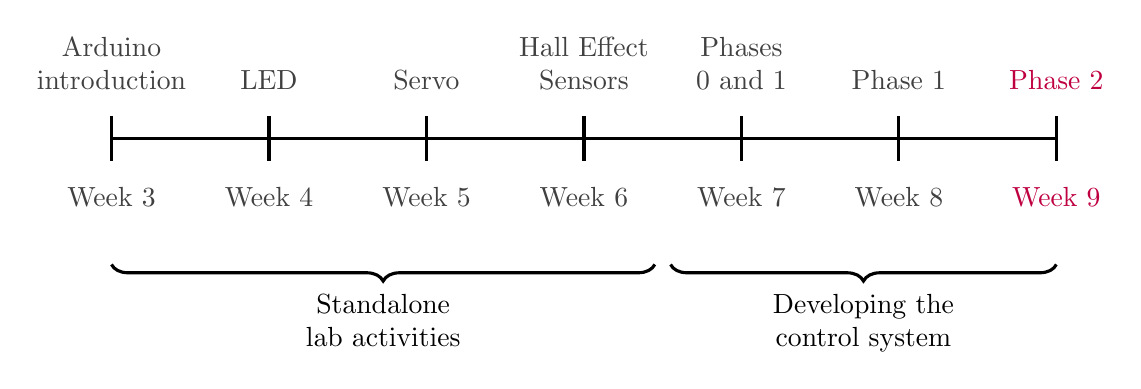
\begin{tikzpicture}[
            timeline/.style={color=black, line width=0.4mm},
            pastnode/.style={align=center, color=darkgray},
            currentnode/.style={align=center, color=purple},
            futurenode/.style={align=center, color=black}
        ]
            %line
            \draw[timeline] (-6, 0) -- (6, 0);

            % week ticks
            \foreach \x in {-6, -4, -2, 0, 2, 4, 6}{
                \draw[timeline] (\x, -0.28) -- (\x, 0.28);
            }

            % weeks (below the line)
            \node[pastnode, below] at (-6, -0.5) {Week 3};
            \node[pastnode, below] at (-4, -0.5) {Week 4};
            \node[pastnode, below] at (-2, -0.5) {Week 5};
            \node[pastnode, below] at (0, -0.5) {Week 6};
            \node[pastnode, below] at (2, -0.5) {Week 7};
            \node[pastnode, below] at (4, -0.5) {Week 8};
            \node[currentnode, below] at (6, -0.5) {Week 9};

            % activities (above the line)
            \node[pastnode, above] at (-6, 0.5) {Arduino\\introduction};
            \node[pastnode, above] at (-4, 0.5) {LED};
            \node[pastnode, above] at (-2, 0.5) {Servo};
            \node[pastnode, above] at (0, 0.5) {Hall Effect\\Sensors};
            \node[pastnode, above] at (2, 0.5) {Phases\\0 and 1};
            \node[pastnode, above] at (4, 0.5) {Phase 1};
            \node[currentnode, above] at (6, 0.5) {Phase 2};

            % phases
            \draw[timeline, decorate, decoration={brace, amplitude=6pt, mirror}] (-6, -1.6) -- (0.9, -1.6);
            \node[futurenode, below] at (-2.55, -1.85) {Standalone\\lab activities};
            \draw[timeline, decorate, decoration={brace, amplitude=6pt, mirror}] (1.1, -1.6) -- (6, -1.6);
            \node[futurenode, below] at (3.55, -1.85) {Developing the \\ control system};

        \end{tikzpicture}
    \end{center}
\end{frame}

\begin{frame}{Today}
    \Large
    Everything is built and tested. Today: how good is the example controller, and how could you make it better?

    \vspace{1em}
    Not finished step 5 yet? Do that first.
\end{frame}

\begin{frame}{Testing the example controller}
    \Large
    \textbf{Predict}: sketch the motor demand and the wheel speed against time.

    \vspace{1em}
    \textbf{Test}: turn the crank about once a second for 20 seconds, then stop.

    \vspace{1em}
    \textbf{Compare}: copy the serial monitor output and plot it. Does it match your sketch?
\end{frame}

% the worksheet's figure, one panel per slide: the top panel (demand) and
% then the bottom panel (speed), cropped from the same pdf
\begin{frame}{What we want vs what we get: motor demand}
    \begin{center}
        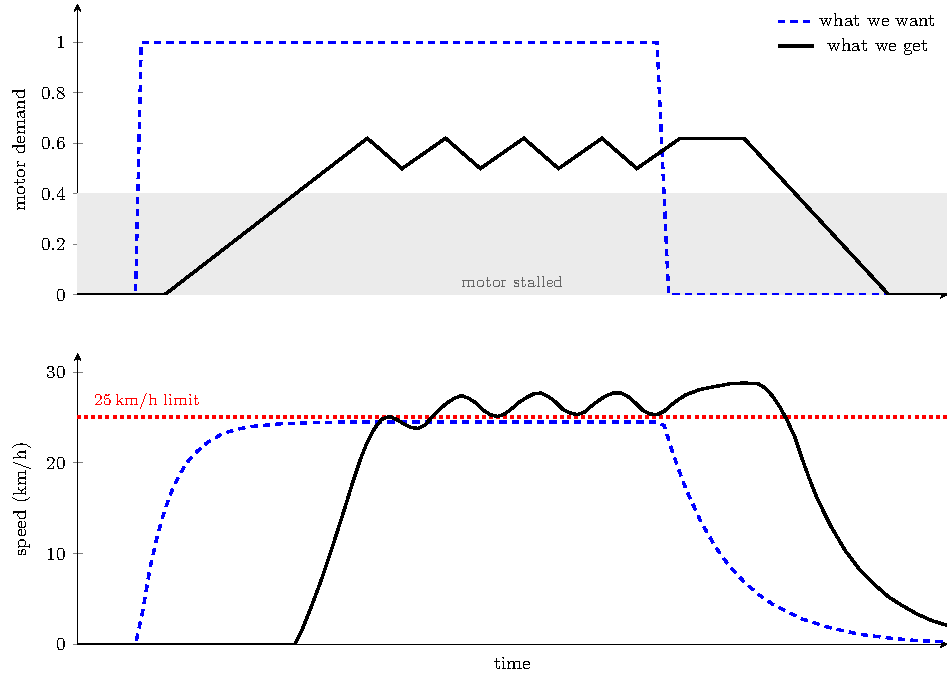
\includegraphics[width=\textwidth, trim=0 172pt 0 0, clip]{want-vs-get.pdf}
    \end{center}
\end{frame}

\begin{frame}{What we want vs what we get: speed}
    \begin{center}
        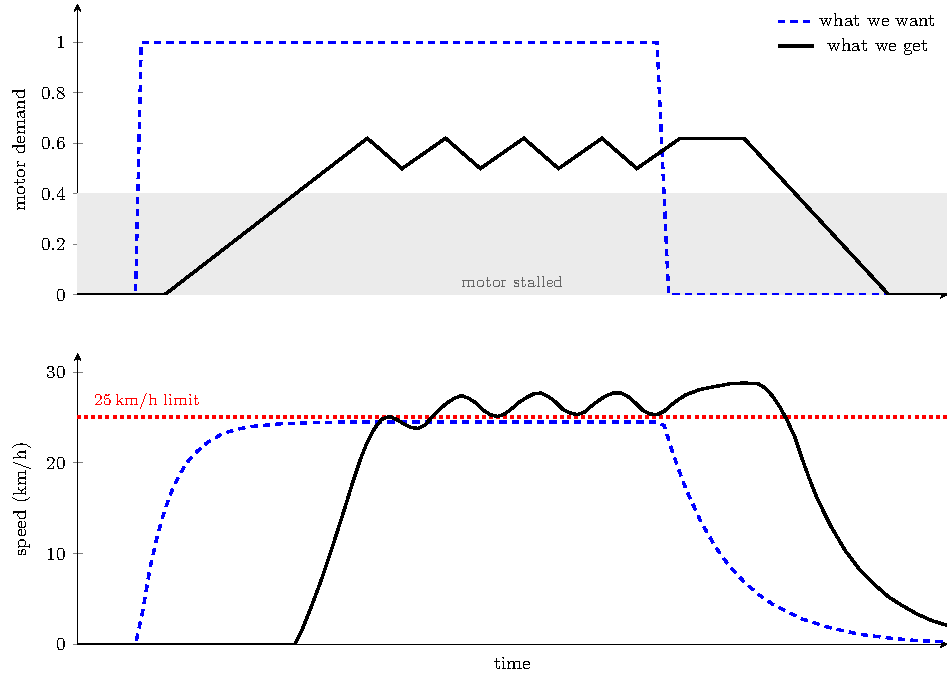
\includegraphics[width=\textwidth, trim=0 0 0 155pt, clip]{want-vs-get.pdf}
    \end{center}
    \small
    Dashed: what we want. Solid: what we get.
\end{frame}

\begin{frame}{Three problems}
    \Large
    \textbf{Slow start}: the motor stalls until the demand reaches about 0.4.

    \vspace{1em}
    \textbf{Overshoot}: the speed wobbles around the 25\,km/h limit.

    \vspace{1em}
    \textbf{Late stop}: the help carries on for up to 3 seconds after the rider stops.
\end{frame}

\begin{frame}{Your turn}
    \Large
    Change anything between the two lines of slashes in `loop'. Leave the \texttt{DO NOT CHANGE} block alone.

    \vspace{1em}
    \large
    \begin{itemize}
        \setlength{\itemsep}{.5em}
        \item Start the ramp from where your motor starts to turn.
        \item Ease off as the bike gets close to 25\,km/h.
        \item Change the ramp rates.
    \end{itemize}

    \vspace{1em}
    \Large
    Same method as Phase 1: one change at a time, predict, test, compare.
\end{frame}

\begin{frame}{Help}
    \normalsize
    \begin{columns}
        \begin{column}{.5\textwidth}
            \begin{center}
                \textbf{Worksheet}\\
                \vspace{.5em}
                \qrcode[hyperlink, height=3cm]{https://github.com/MDCHAMP/MAC233/blob/main/control-system/docs/control-system.pdf}
            \end{center}
        \end{column}
        \begin{column}{.5\textwidth}
            \begin{center}
                \textbf{Sketch}\\
                \vspace{.5em}
                \qrcode[hyperlink, height=3cm]{https://github.com/MDCHAMP/MAC233/blob/main/control-system/control-system.ino}
            \end{center}
        \end{column}
    \end{columns}

    \vspace{3.5em}
    Problems? Raise your hand and someone will come and help you.
\end{frame}

\end{document}
